\begin{frame}{Kiến trúc RAG - Giai đoạn Truy xuất và Tạo sinh}
\begin{figure}[H]
\centering
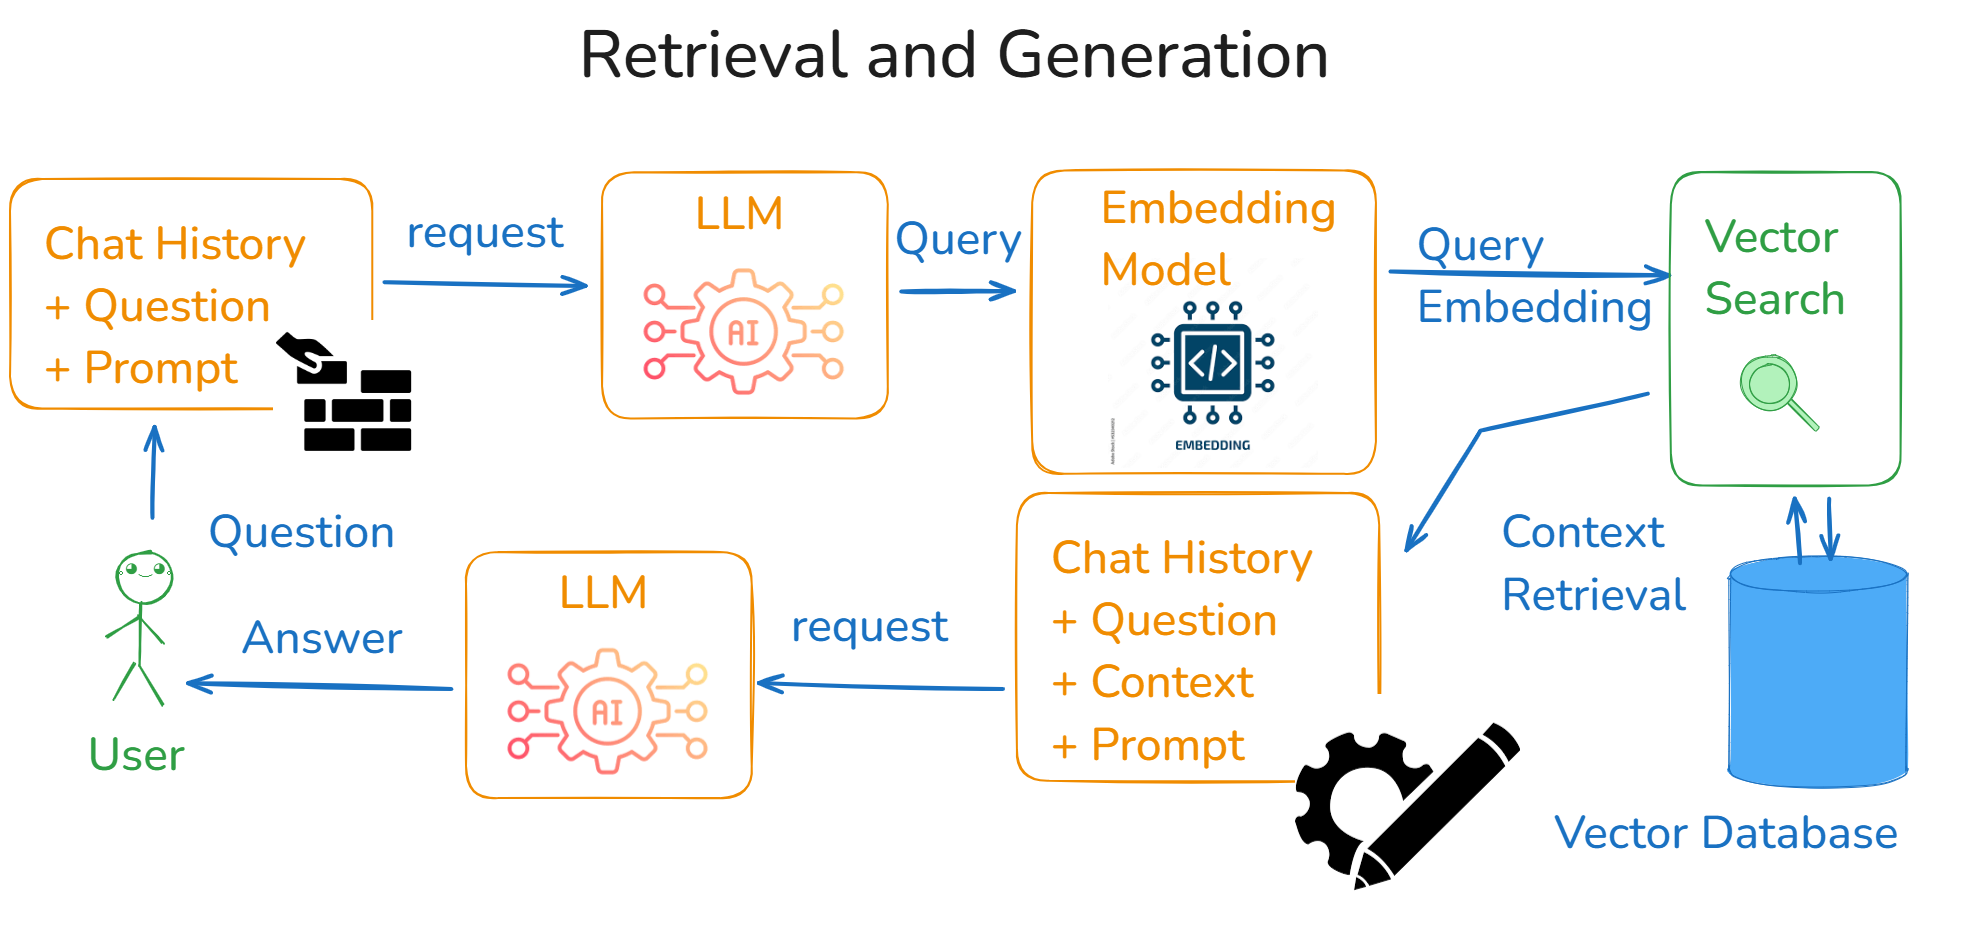
\includegraphics[height=0.55\textheight,width=0.9\textwidth,keepaspectratio]{pictures/rag-2.excalidraw.png}
\caption{Sơ đồ RAG cơ bản (Retrieval and Generation)}
\end{figure}

\note{
Giai đoạn thứ hai của RAG là Truy xuất (Retrieval) và Tạo sinh (Generation).
Khi người dùng gửi câu hỏi, hệ thống vector hóa câu hỏi và truy xuất các đoạn tài liệu liên quan nhất từ Vector Database.
Các đoạn tài liệu này được làm giàu vào prompt làm ngữ cảnh cho LLM. LLM sử dụng ngữ cảnh đó để sinh ra câu trả lời chính xác và đáng tin cậy đối với nguồn dữ liệu, hạn chế hiện tượng ảo giác.
}
\end{frame}
